\begin{figure}[h]
\centering
\begin{subfigure}[b]{0.3\textwidth}
    \centering
    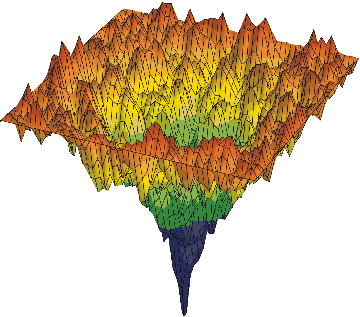
\includegraphics[width=\textwidth]{figures/drysurf.png}
    \label{fig:dry}
    \caption{}
\end{subfigure}%
\hspace{0.1\textwidth}
\begin{subfigure}[b]{0.3\textwidth}
    \centering
    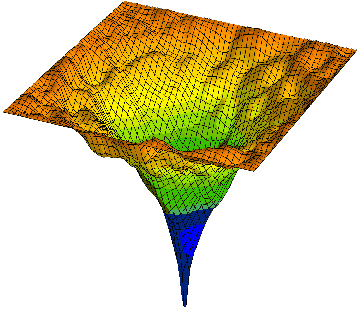
\includegraphics[width=\textwidth]{figures/wetsurf.png}
    \label{fig:wet}
    \caption{}
\end{subfigure}
\caption{
Here energy is represented as a function of the two principal components of the protein conformation.
In both cases, the approximate funnel shape of the energy surface about the native conformation is very apparent.
(a) An energy surface without any solvent effects contains a large number of local minima giving the surface a jagged appearance.
(b) A surface including hydration effects appears smooth relative to the dry surface, due to water providing a source of hydrogen bond donors and acceptors such that hydrogen bonds are possible in many side chain conformations.
In reality all energy landscapes of larger proteins contain many local minima.
Figure from \protect\cite{waterwebsite}, used with author's permission.
}
\label{fig:funnel}
\end{figure}

The potential energy barriers are lowered and smoothed due to the ease with which water molecules can lubricate the movement of the amino acid backbone and side groups by the rapid formation and exchange of hydrogen bonds
